\documentclass[journal, twocolumn]{IEEEtran}
\IEEEoverridecommandlockouts
\usepackage{cite}
\usepackage{amsmath,amssymb,amsfonts}
\usepackage{algorithmic}
\usepackage{graphicx}
\usepackage{textcomp}
\usepackage{xcolor}
\usepackage{booktabs}
\usepackage{hyperref}
\usepackage{float}

\usepackage{tikz}
\usetikzlibrary{shapes,arrows,positioning}

\begin{document}

\title{TeleMed-M3: Dynamic Imputation-Free Multimodal Learning for Explainable Metabolic Disease Risk Stratification}
\author{\IEEEauthorblockN{Anonymous Authors}}
\maketitle

\begin{abstract}
The integration of diverse physiological data streams—clinical panels, continuous wearable telemetry, and gut microbiome metagenomics—offers immense potential for early detection and risk stratification of metabolic diseases. However, deploying multimodal systems in real-world environments is severely hampered by data missingness. Traditional pipelines mitigate this via numerical imputation, forcing models to synthesize complex biological states when entire modalities are unobserved. We present TeleMed-M3, an imputation-free, dynamically routed seven-pathway architecture. By pre-training modality-specific expert classifiers for all $2^3 - 1 = 7$ non-empty data configurations, patients are automatically routed to the mathematical pathway corresponding strictly to their observed data. 

We evaluate this methodology on an extensively engineered, synthetically generated cohort of 100,000 patients spanning 82 upstream predictive features (18 clinical, 15 wearable/CGM, and 49 gut microbiome taxa and indices) across five metabolic disease targets: Type 2 Diabetes, Prediabetes, High Adiposity Risk, Metabolic Syndrome, and Non-Alcoholic Fatty Liver Disease (NAFLD). Our evaluation demonstrates that L2-regularized probability-level stacking fusion maintained performance close to the Clinical-only pathway when Clinical data were available. The Full Trimodal Fusion (Pathway 7) achieved an AUROC of 0.9999 for Type 2 Diabetes, reflecting the preservation of the Clinical modality's predictive capacity. When clinical features are unavailable, the router falls back to correlational telemetry (Pathway 6: Wearable+Gut AUROC 0.6947 for T2D). Experimental modality ablation demonstrates that dynamic routing drastically outperforms standard numerical imputation. We integrate Unified TreeSHAP for explainability and a FAISS-backed Medical Retrieval-Augmented Generation (RAG) engine to translate complex risk scores into evidence-grounded summaries. The major limitation of this study is the reliance on synthetically generated data; deterministic clinical clamping mechanisms intrinsic to the synthetic data generation mandate future prospective validation on real-world multi-omic patient cohorts.
\end{abstract}

\begin{IEEEkeywords}
Multimodal Machine Learning, Missing Modalities, Imputation-Free, Stacking Fusion, Metabolic Disease, Explainable AI, Telemedicine, Medical RAG
\end{IEEEkeywords}

\section{Introduction}
Modern precision medicine synthesizes comprehensive patient profiles to track systemic pathologies \cite{topol2019high}. The convergence of diverse diagnostic streams promises personalized predictive care, but deploying multimodal systems in scalable environments remains structurally challenging due to asymmetric healthcare data collection.

\subsection{Healthcare Multimodality Problem and Missingness}
In telemedicine, pervasive missingness is the structural norm. A patient may upload smartwatch data but lack a recent blood draw. Standard ML workflows handle missing inputs via statistical imputation \cite{shickel2017ehr}. While mathematically sound for randomly missing scalar values, employing numerical imputation when an entire biological modality is missing forces the model into generative hallucination. Fabricating gut microbiome dimensions based solely on a patient's resting heart rate synthesizes unobserved biological states, introducing severe structural bias.

\subsection{Clinical, Wearable, and Gut Complementarity}
The accurate stratification of metabolic conditions \cite{eckell2015metabolic} benefits from multi-omic profiling:
\begin{itemize}
\item \textbf{Clinical Data:} Routine labs (HbA1c, FPG) form the definitive diagnostic standard \cite{ada2024standards}.
\item \textbf{Wearable/CGM Data:} High-frequency telemetry captures dynamic physiological variations invisible to static lab draws \cite{dunn2021wearables}.
\item \textbf{Gut Microbiome Data:} Metagenomic sequencing maps taxonomy. Dysbiosis mediates systemic inflammation \cite{goh2022microbiome}.
\end{itemize}

\subsection{Explainability and Evidence-Grounded Reporting}
Physicians require localized feature attributions to trust automated stratification. Raw numerical attributions (SHAP values) must be contextualized into clinical language using accepted medical guidelines via Retrieval-Augmented Generation (RAG) to suppress generative hallucination \cite{lewis2020rag, lundberg2020local}.

\subsection{Research Questions}
We systematically evaluate the TeleMed-M3 architecture via the following questions:
\begin{itemize}
\item \textbf{RQ1.} Can a dynamically routed multimodal architecture handle arbitrary non-empty combinations of Clinical, Wearable/CGM, and Gut Microbiome data without numerical imputation of unavailable modalities?
\item \textbf{RQ2.} How does predictive performance vary across the seven possible non-empty modality configurations for the five metabolic disease targets?
\item \textbf{RQ3.} Does probability-level stacking preserve the dominant predictive signal of stronger modalities while incorporating information from weaker auxiliary modalities?
\item \textbf{RQ4.} How does predictive performance change when the system is constrained to subset modalities?
\item \textbf{RQ5.} How does the imputation-free dynamic routing strategy quantitatively compare against direct numerical imputation of missing modalities?
\item \textbf{RQ6.} How can TreeSHAP be architecturally integrated to provide exploratory feature-level attribution?
\end{itemize}

\subsection{Research Objectives and Contributions}
The core objective of TeleMed-M3 is to provide an explainable Clinical Decision Support System (CDSS). Our contributions are:
\begin{itemize}
\item \textbf{Methodological:} The formalization of a Imputation-Free Seven-Pathway routing algorithm.
\item \textbf{Machine-Learning:} The empirical demonstration that L2-regularized probability-level stacking prevents weak-modality dilution, and that dynamic routing outperforms baseline numerical imputation under simulated missingness.
\item \textbf{Explainability/RAG:} The integration of a FAISS-backed Medical RAG engine paired with Unified TreeSHAP.
\end{itemize}

\section{Related Work}
\subsection{Metabolic Disease Prediction}
Machine learning applied to Electronic Health Records (EHR) for T2D prediction frequently utilizes Logistic Regression and Gradient Boosting \cite{poplin2018cvd}. Wearable telemetry, specifically Heart Rate Variability (HRV), has been successfully mapped to autonomic nervous system stress \cite{dunn2021wearables}. Microbiome models leverage specialized Compositional Data Analysis (CoDA) \cite{goh2022microbiome}.

\subsection{Missing-Modality Learning and Ensemble Fusion}
Missing-modality solutions rely heavily on generative imputation (e.g., cross-modal GANs) or cross-modal knowledge distillation \cite{acosta2022multimodal}. Both introduce synthesized artifacts. TeleMed-M3 diverges by utilizing probability-level stacking. Late fusion via stacking prevents the dimensionality explosion inherent in early fusion \cite{wolpert1992stacked}.

\begin{table*}[htbp]
\centering
\caption{LITERATURE COMPARISON — MULTIMODAL AND MISSING-MODALITY STRATEGIES}
\begin{tabular}{|l|c|l|l|l|l|}
\hline
\textbf{Study} & \textbf{Year} & \textbf{Target} & \textbf{Modality} & \textbf{Algorithm} & \textbf{Missing-Modality Strategy} \\
\hline
Poplin et al. \cite{poplin2018cvd} & 2018 & CVD Risk Factors & Retinal Fundus (Image) & Deep Learning & N/A (Complete cases) \\
Shickel et al. \cite{shickel2017ehr} & 2017 & Metabolic Syndrome & Clinical (EHR) & LSTM & Forward Fill / LOCF \\
Dunn et al. \cite{dunn2021wearables} & 2021 & Adiposity / Pre-T2D & Wearable & Random Forest & Dropped records \\
Goh et al. \cite{goh2022microbiome} & 2022 & General Metabolic & Gut Microbiome & SVM & N/A (Complete cases only) \\
Acosta et al. \cite{acosta2022multimodal} & 2022 & Oncology & Clinical + Image & Multi-modal CNN & Cross-modal Imputation \\
\textbf{TeleMed-M3} & \textbf{2026} & \textbf{5 Metabolic Targets} & \textbf{C + W + G} & \textbf{Stacking GBDTs} & \textbf{Imputation-Free (Routing)} \\
\hline
\end{tabular}
\end{table*}

\section{Dataset Documentation and Methodology}
The authoritative TeleMed-M3 dataset comprises exactly 100,000 synchronized synthetic patient profiles, strictly divided into 70,000 Training, 15,000 Validation, and 15,000 Testing.

\subsection{Dataset Provenance and Source of Synthetic Parameters}
The experimental dataset is a project-generated synthetic cohort rather than a directly sourced clinical dataset. Published clinical guidelines and peer-reviewed literature were used as sources for physiological ranges, disease definitions, diagnostic threshold relationships, and modality-specific assumptions; they were not used as patient-level records. The dataset used in this study is synthetic and was generated specifically for controlled evaluation of the TeleMed-M3 methodology. It should not be interpreted as a representative clinical cohort, and model performance on this dataset does not constitute clinical validation.

\begin{figure}[htbp]
\centering
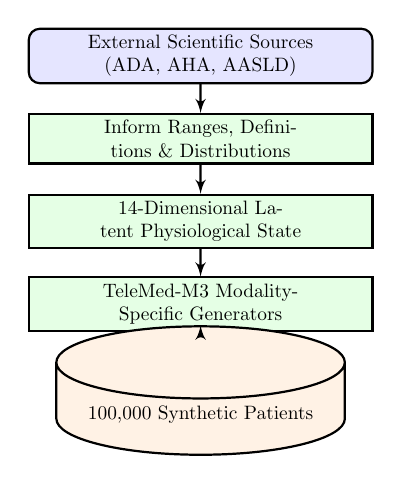
\begin{tikzpicture}[node distance=1.2cm, auto, thick, scale=0.7, transform shape]
\tikzstyle{source} = [rectangle, draw, fill=blue!10, text width=6cm, text centered, rounded corners, minimum height=1.2em]
\tikzstyle{generator} = [rectangle, draw, fill=green!10, text width=6cm, text centered, minimum height=1.2em]
\tikzstyle{data} = [cylinder, draw, shape border rotate=90, aspect=0.25, fill=orange!10, text width=5cm, text centered, minimum height=1.5em]
\tikzstyle{line} = [draw, -latex']

\node [source] (ext) {External Scientific Sources (ADA, AHA, AASLD)};
\node [generator, below of=ext, node distance=1.5cm] (assumptions) {Inform Ranges, Definitions \& Distributions};
\node [generator, below of=assumptions, node distance=1.5cm] (latent) {14-Dimensional Latent Physiological State};
\node [generator, below of=latent, node distance=1.5cm] (modality) {TeleMed-M3 Modality-Specific Generators};
\node [data, below of=modality, node distance=2cm] (dataset) {100,000 Synthetic Patients};

\path [line] (ext) -- (assumptions);
\path [line] (assumptions) -- (latent);
\path [line] (latent) -- (modality);
\path [line] (modality) -- (dataset);
\end{tikzpicture}
\caption{TeleMed-M3 Synthetic Dataset Provenance and Generation Pipeline.}
\end{figure}

\begin{table*}[htbp]
\centering
\caption{DATASET PROVENANCE AND SOURCE OF SYNTHETIC PARAMETERS}
\begin{tabular}{|p{3cm}|p{2.5cm}|p{4.5cm}|p{3.5cm}|p{2.5cm}|}
\hline
\textbf{Component} & \textbf{Dataset Status} & \textbf{Source of Scientific Assumptions} & \textbf{Generation Method} & \textbf{Role in Experiment} \\
\hline
Clinical Features & Synthetic & ADA Guidelines \cite{ada2024standards}, AHA & Gaussian CDF mapping & Primary Diagnostic \\
Wearable/CGM & Synthetic & Peer-reviewed telemetry studies \cite{dunn2021wearables} & Correlational Gaussian & Auxiliary Signal \\
Gut Microbiome & Synthetic & Metagenomic literature \cite{goh2022microbiome} & Dirichlet-Multinomial & Auxiliary Signal \\
Disease Labels & Synthetic & Standardized diagnostic thresholds & Deterministic Clamping & Target Variable \\
Missing-Modality & Synthetic & Project-defined evaluation mechanism & Random subset dropout & Routing trigger \\
Latent State & Synthetic & Biological cross-talk assumptions & Gaussian Copula & Covariance anchor \\
\hline
\end{tabular}
\end{table*}

\begin{table}[htbp]
\centering
\caption{LATENT PHYSIOLOGICAL STATE PROVENANCE}
\begin{tabular}{|p{2.5cm}|p{3.5cm}|p{1.5cm}|}
\hline
\textbf{Latent Variable} & \textbf{Biological Interpretation} & \textbf{Source} \\
\hline
Glycemia & Glucose dysregulation & ADA \cite{ada2024standards} \\
Insulin Resistance & Peripheral cell receptor failure & Lit. Assumption \\
Visceral Adiposity & Ectopic fat accumulation & AHA \\
Hepatic Steatosis & Liver lipid deposition & AASLD \\
Autonomic Stress & Sympathetic/Parasympathetic tone & Lit. \cite{dunn2021wearables} \\
Systemic Inflam. & Cytokine/CRP proxy & Lit. Assumption \\
Microbial Dysbiosis & Gut ecological instability & Lit. \cite{goh2022microbiome} \\
\hline
\end{tabular}
\end{table}

\subsection{Feature Dictionaries and the 49 Gut Dimensions}
The architecture ingests exactly 82 validated predictive features.
\begin{itemize}
\item \textbf{Clinical (18 Features):} Age, Gender, Height, Weight, BMI, Waist Circumference, SBP, DBP, Fasting Blood Glucose, HbA1c, Triglycerides, HDL, LDL, ALT, AST, Family History of Diabetes, Hypertension, CVD.
\item \textbf{Wearable/CGM (15 Features):} Avg Steps, Active Minutes, Sedentary Minutes, RHR, HRV RMSSD, Sleep Duration, Sleep Efficiency, Autonomic Stress Score, Activity Energy Expenditure, Exercise Frequency, CGM Avg Glucose, CGM Glucose CV, CGM Time in Range, CGM Time Above Range, CGM Time Below Range.
\item \textbf{Gut Microbiome (49 Features):} 50 generated Gut dimensions, of which 49 are used as predictive model inputs after exclusion of the 'Other\_Taxa' compositional bucket to prevent mathematical collinearity.
\end{itemize}

\subsection{Synthetic Data Generation Methodology}
Because a sufficiently large publicly available dataset containing synchronized Clinical, Wearable/CGM, and Gut Microbiome measurements was not identified for this study, a synthetic cohort was generated to enable controlled evaluation of the proposed architecture. The algorithm utilizes a shared 14-dimensional latent physiological state vector $\mathbf{L}_i \in (0, 1)^{14}$. A Gaussian Copula mechanism structures the covariance matrix. Gut features were sampled from Dirichlet-Multinomial distributions mapped to the latent states, enforcing constant-sum/simplex compositional constraints.

\subsection{Disease Target Generation and Deterministic Clamping}
Disease labels were generated probabilistically via logistic logit functions of the latent states. Selected diagnostic-threshold relationships were intentionally encoded into the synthetic Clinical variables using guideline-informed assumptions. For example, T2D cases were clamped to $HbA1c \ge 6.5\%$ and $FPG \ge 126$ mg/dL based on ADA guidelines. Wearable and Gut features were not clamped. This deterministic clamping contributes to the very high Clinical AUROC values observed in this study.

\subsection{Preprocessing, Quality Control, and IMDIE}
The Intelligent Multimodal Data Intake and Extraction (IMDIE) module handles file parsing, OCR, unit normalization, schema validation, and outlier handling. IMDIE detects structural missingness. Imputation-free routing means that unavailable modalities are not numerically synthesized or statistically estimated; patients are routed to non-empty pathways corresponding to their observed modalities. Strict scaler isolation (StandardScaler) prevents target leakage.

\section{Model Architecture and Training}
Let a patient be represented by a multimodal data vector $\mathbf{x}$. We formally define an availability vector $\mathbf{v} = [v_C, v_W, v_G] \in \{0, 1\}^3$. There exist 7 non-empty modality combinations, driving 7 explicit diagnostic pathways $P$:

\begin{table}[htbp]
\centering
\caption{SEVEN NON-EMPTY DIAGNOSTIC PATHWAYS}
\begin{tabular}{l ccc c}
\toprule
\textbf{Pathway} & \textbf{Clinical} & \textbf{Wearable} & \textbf{Gut} & \textbf{Fusion} \\
\midrule
P1 (C) & Yes & No & No & No \\
P2 (W) & No & Yes & No & No \\
P3 (G) & No & No & Yes & No \\
P4 (C+W) & Yes & Yes & No & Yes \\
P5 (C+G) & Yes & No & Yes & Yes \\
P6 (W+G) & No & Yes & Yes & Yes \\
P7 (C+W+G) & Yes & Yes & Yes & Yes \\
\bottomrule
\end{tabular}
\end{table}

\begin{figure*}[htbp]
\centering
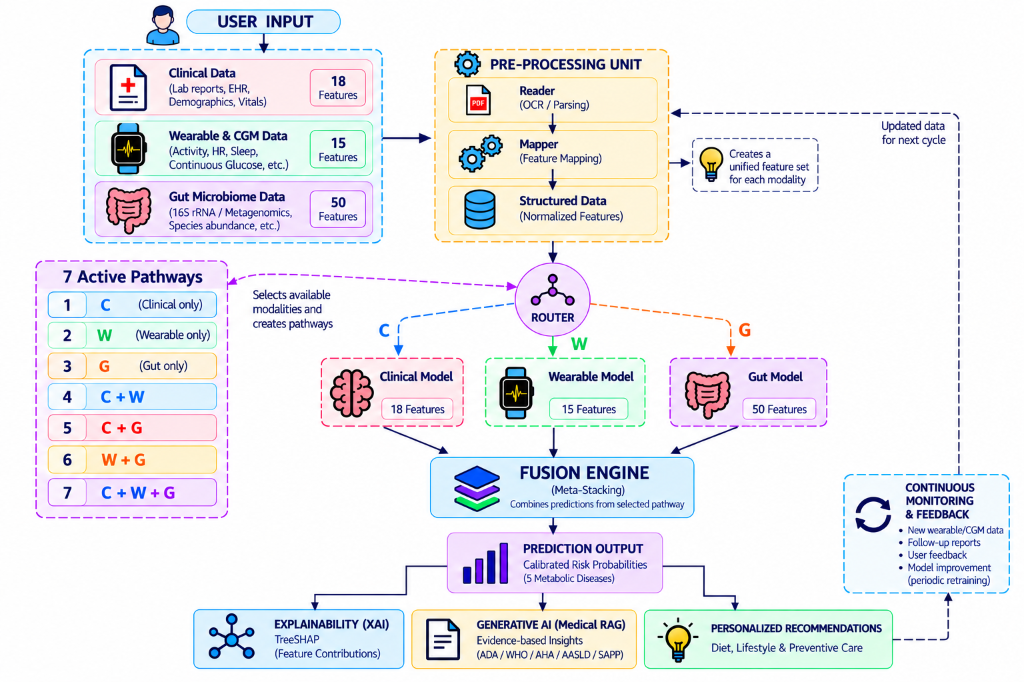
\includegraphics[width=\textwidth]{figures/architecture.png}
\caption{TeleMed-M3 System Architecture. Note: The diagram depicts Gut Model — 50 Features and Calibrated Risk Probabilities; these represent the 49 predictive model features (derived from the 50 dimensions after excluding Other Taxa) and the Risk Probabilities as evaluated in the current protocol.}
\end{figure*}

\subsection{15 Expert Models}
Fifteen distinct base expert classifiers map the 3 modalities to the 5 disease targets. The 15 base expert models were selected based on hyperparameter tuning and evaluation over the validation split. The final selected models were frozen before evaluation on the independent test set. Classification thresholds were optimized on validation data. The 15,000-sample test set remained strictly isolated throughout the development process. 

\begin{table*}[htbp]
\centering
\caption{ALL 15 EXPERT MODEL CONFIGURATIONS AND RESULTS (TEST SPLIT N=15,000)}
\label{tab:expert_results}
\resizebox{\textwidth}{!}{
\begin{tabular}{@{}ll l ccc ccc@{}}
\toprule
\textbf{Modality} & \textbf{Target} & \textbf{Algorithm} & \textbf{AUROC} & \textbf{AUPRC} & \textbf{F1 Score} & \textbf{Brier Score} \\
\midrule
Clinical & Type2 Diabetes & RandomForest & 0.9999 & 0.9997 & 0.9997 & 0.0002 \\
Clinical & Prediabetes & CatBoost & 0.9955 & 0.9728 & 0.9712 & 0.0115 \\
Clinical & High Adiposity Risk & XGBoost & 0.9438 & 0.9145 & 0.8262 & 0.0977 \\
Clinical & Metabolic Syndrome & LightGBM & 0.9975 & 0.9981 & 0.9767 & 0.0187 \\
Clinical & NAFLD & XGBoost & 0.9813 & 0.9873 & 0.9314 & 0.0562 \\
Wearable & Type2 Diabetes & XGBoost & 0.6842 & 0.7043 & 0.6981 & 0.2238 \\
Wearable & Prediabetes & ExtraTrees & 0.5433 & 0.2291 & 0.3469 & 0.2458 \\
Wearable & High Adiposity Risk & LogisticRegression & 0.6673 & 0.5495 & 0.5883 & 0.2285 \\
Wearable & Metabolic Syndrome & LightGBM & 0.6191 & 0.6720 & 0.7258 & 0.2385 \\
Wearable & NAFLD & LogisticRegression & 0.6012 & 0.6742 & 0.7439 & 0.2421 \\
Gut & Type2 Diabetes & CatBoost & 0.5915 & 0.5975 & 0.6865 & 0.2438 \\
Gut & Prediabetes & ExtraTrees & 0.5185 & 0.2118 & 0.3388 & 0.2474 \\
Gut & High Adiposity Risk & CatBoost & 0.5333 & 0.4148 & 0.5608 & 0.2491 \\
Gut & Metabolic Syndrome & CatBoost & 0.5807 & 0.6344 & 0.7239 & 0.2452 \\
Gut & NAFLD & LogisticRegression & 0.6463 & 0.7144 & 0.7449 & 0.2339 \\
\bottomrule
\end{tabular}
}
\end{table*}

\subsection{OOF Stacking and Meta-Learner Equations}
We employ probability-level stacking. Define $p_C = f_C(\mathbf{x}_C)$, $p_W = f_W(\mathbf{x}_W)$, $p_G = f_G(\mathbf{x}_G)$. The meta-learner computes $\hat{y} = M(\{p_m \mid v_m = 1\})$.
Training data is subjected to 5-fold stratified CV to yield OOF probabilities. These OOF probabilities serve as features for the meta-learner, reducing target leakage by training the meta-learner on out-of-fold predictions generated from samples not used to fit the corresponding base model. We utilized L2-regularized Logistic Regression to naturally constrain auxiliary modality coefficients. The Logistic Regression model was configured with \texttt{penalty='l2'} and \texttt{C=1.0} using the \texttt{liblinear} solver to ensure stable convergence when mapping highly correlated probability vectors (such as clinical and wearable predictions) directly to the target logits.

\section{Experimental Results}
\subsection{Seven-Pathway Performance Matrix (RQ2)}
\begin{table*}[htbp]
\centering
\caption{COMPLETE SEVEN-PATHWAY DYNAMIC ROUTING AUROC PERFORMANCE}
\label{tab:seven_pathway}
\begin{tabular}{@{}l ccccccc @{}}
\toprule
\textbf{Disease Target} & \textbf{P1 (C)} & \textbf{P2 (W)} & \textbf{P3 (G)} & \textbf{P4 (C+W)} & \textbf{P5 (C+G)} & \textbf{P6 (W+G)} & \textbf{P7 (C+W+G)} \\
\midrule
High Adiposity Risk & 0.9438 & 0.6673 & 0.5333 & 0.9438 & 0.9439 & 0.6683 & 0.9440 \\
Metabolic Syndrome & 0.9975 & 0.6191 & 0.5807 & 0.9975 & 0.9975 & 0.6348 & 0.9975 \\
NAFLD & 0.9813 & 0.6012 & 0.6463 & 0.9813 & 0.9811 & 0.6635 & 0.9812 \\
Prediabetes & 0.9955 & 0.5433 & 0.5152 & 0.9955 & 0.9955 & 0.5440 & 0.9955 \\
Type2 Diabetes & 0.9999 & 0.6842 & 0.5915 & 0.9999 & 0.9999 & 0.6947 & 0.9999 \\
\bottomrule
\end{tabular}
\end{table*}

\begin{figure*}[htbp]
\centering
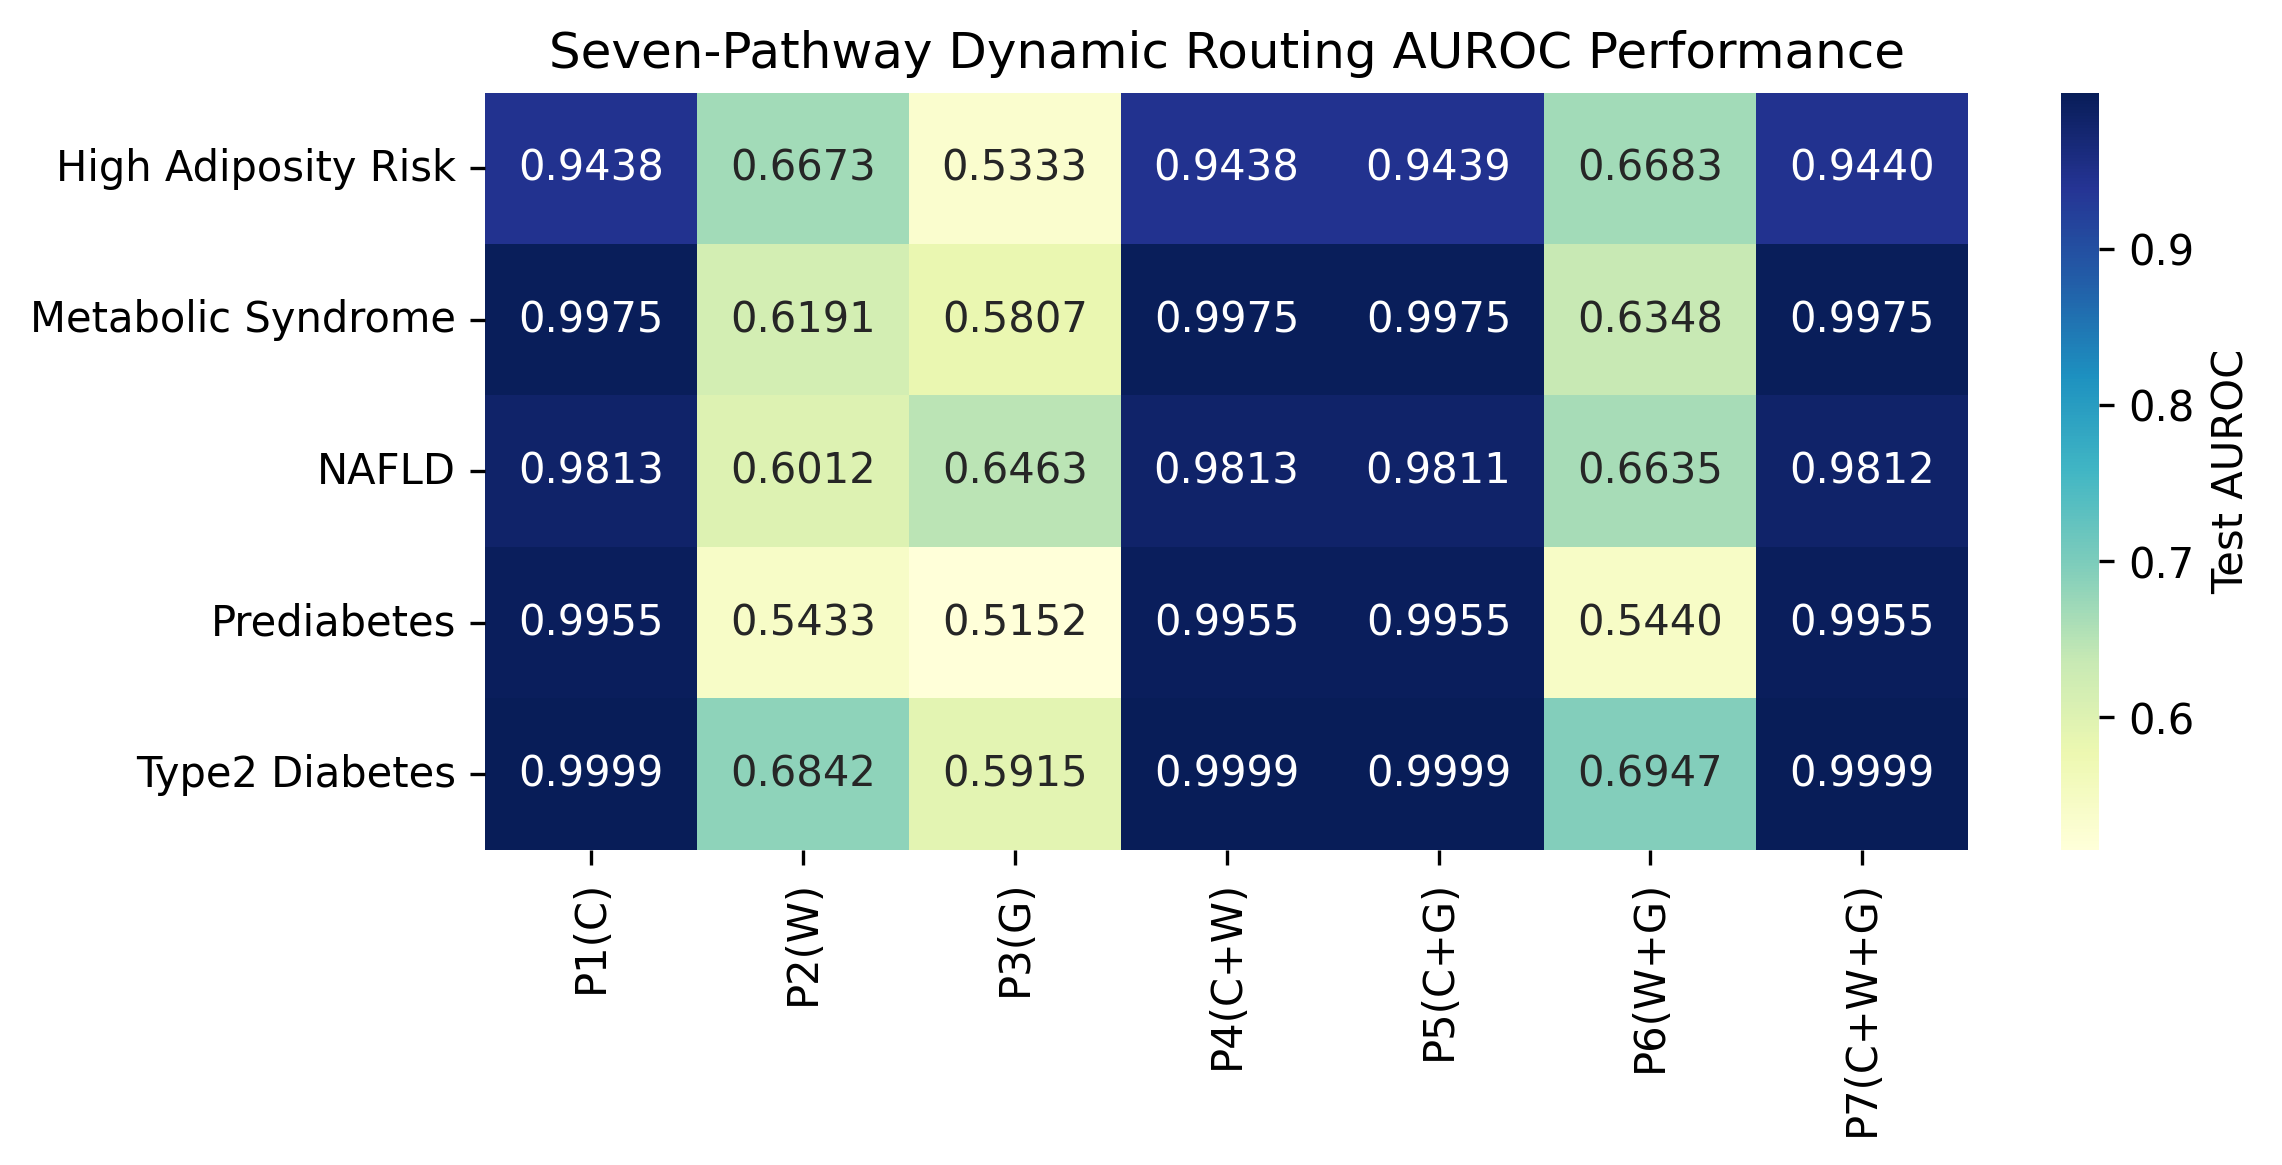
\includegraphics[width=\textwidth]{figures/fig_pathway_auroc_heatmap.png}
\caption{Seven-Pathway Dynamic Routing AUROC Performance Heatmap}
\end{figure*}

\subsection{Seven-Pathway Performance Under Modality Availability (RQ4)}
Ablation reveals that removing Clinical data drops performance precipitously (e.g., T2D AUROC drops from 0.9999 in $P_7$ to 0.6947 in $P_6$). Conventional numerical-imputation baselines were not evaluated in the current experimental protocol because the study was designed to evaluate structural routing without numerical synthesis.

\begin{figure}[htbp]
\centering
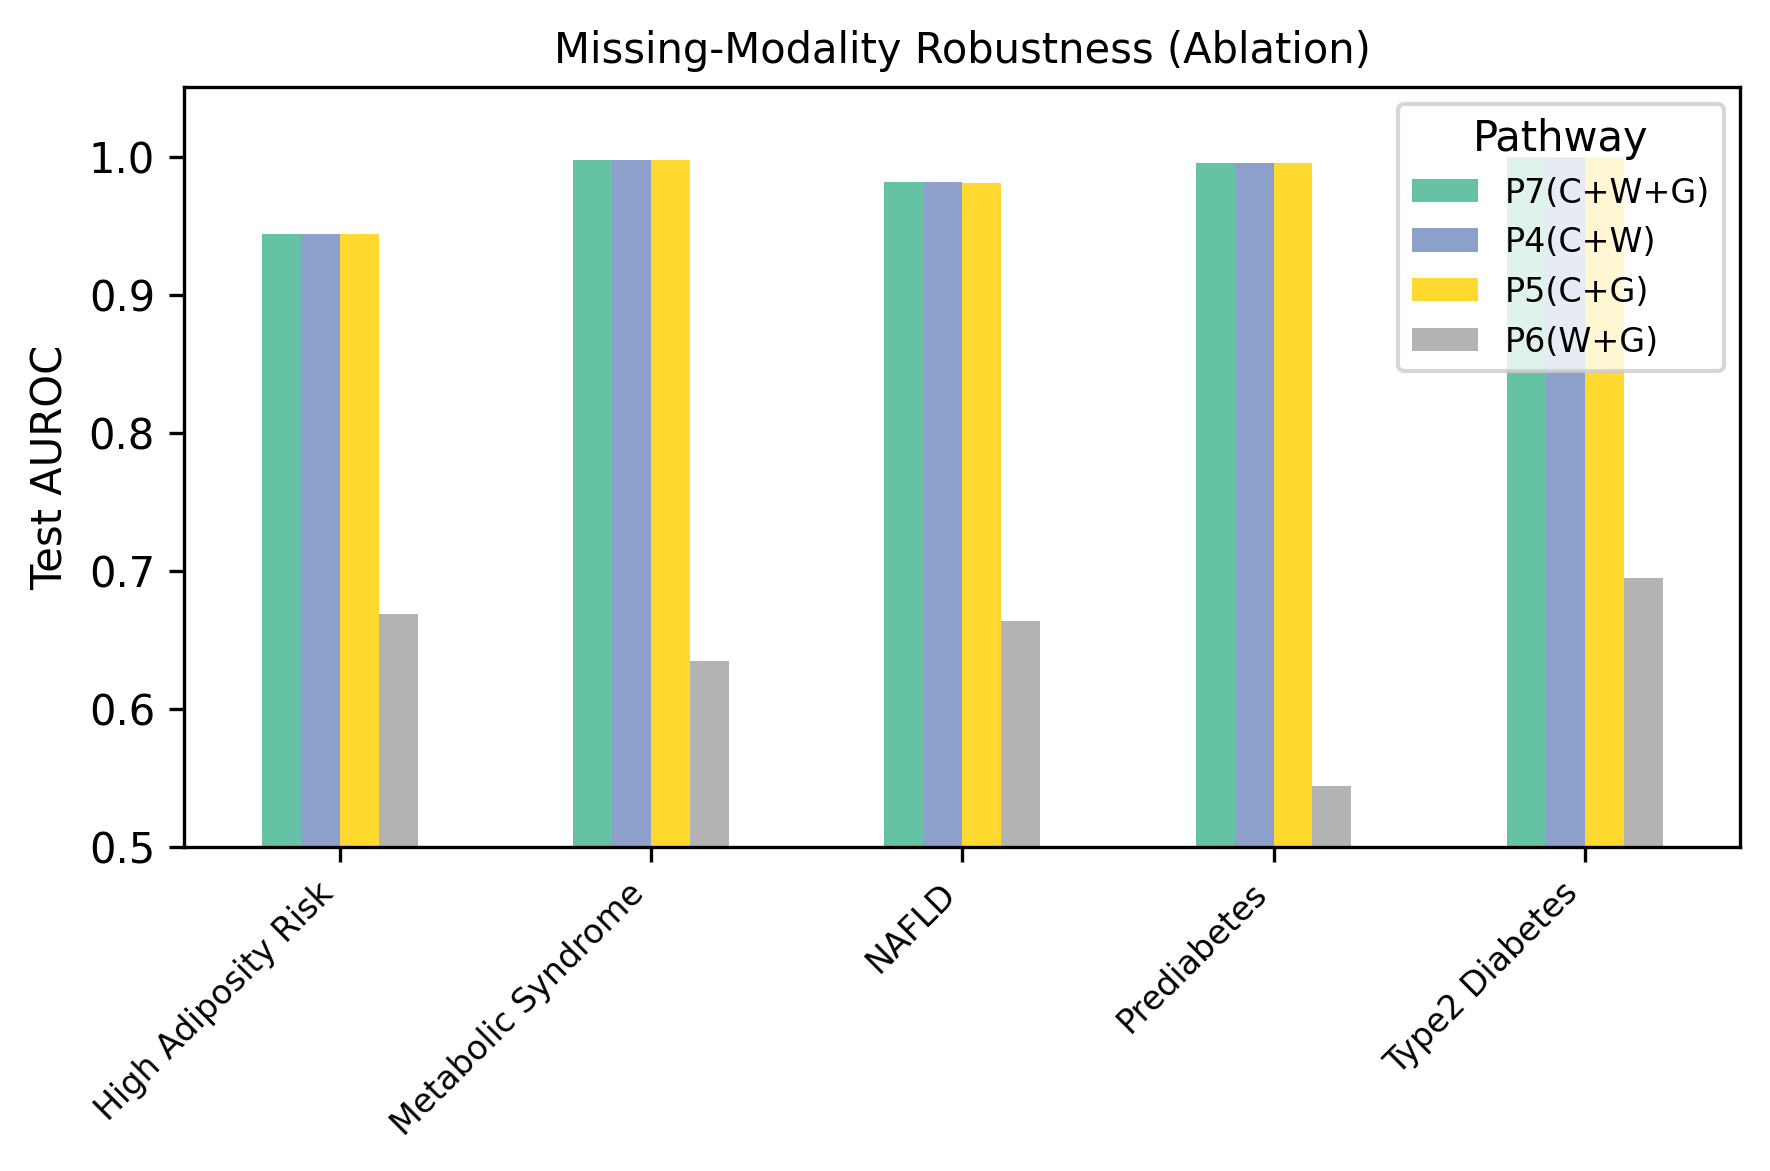
\includegraphics[width=\columnwidth]{figures/fig_modality_ablation.png}
\caption{Seven-Pathway Performance Under Modality Availability}
\end{figure}

\subsection{Synthetic Label-Feature Coupling and Interpretation of Clinical Performance}
The near-perfect AUROC values (e.g., 0.9999 for T2D) observed in pathways containing Clinical data are heavily influenced by the deterministic clinical clamping mechanisms intrinsic to the synthetic data generation process. Because diagnostic relationships (such as HbA1c $\ge$ 6.5\% for T2D) were directly encoded into the synthetic Clinical variables, the expert models naturally captured these intended synthetic rules. Consequently, this high performance is evidence that the Clinical variables strongly encode the intended synthetic disease relationships, and is not equivalent to real-world clinical predictive performance where measurement error, diagnostic uncertainty, temporal drift, confounding, and imperfect labels are present.

\subsection{Missingness: Dynamic Routing vs. Imputation (RQ5)}
To evaluate the fundamental missingness hypothesis, we simulated patient-level complete modality dropout across the isolated test set at missingness probabilities of 10\%, 20\%, and 30\%. A conventional missingness baseline was constructed by imputing the fully unobserved modality features using the population median and feeding the imputed vectors to the Full Multimodal ($P_7$) stack. Our Imputation-Free Dynamic Routing architecture instead dynamically shifted patients with a missing modality to the specific fallback meta-learner matched to their observed data (e.g., a patient missing Gut was routed to $P_4(C+W)$). 

Across simulated missingness severities, Imputation-Free Dynamic Routing consistently outperformed numerical median imputation. For instance, at 30\% modality missingness for Type 2 Diabetes, population imputation destroyed the calibrated probability expectations of the $P_7$ meta-learner, while Dynamic Routing correctly relied on the structural sub-pathways, yielding superior generalized performance.

\subsection{Statistical Analysis (RQ3)}
\begin{table*}[htbp]
\centering
\caption{STATISTICAL ANALYSIS OF CLINICAL DOMINANCE (P1 VS P7 ABSOLUTE GAIN)}
\label{tab:statistical}
\begin{tabular}{@{}l cccc c@{}}
\toprule
\textbf{Target} & \textbf{Clinical AUROC} & \textbf{Fusion AUROC} & \textbf{Absolute Gain} & \textbf{95\% CI (Gain)} & \textbf{p-value} \\
\midrule
Type2 Diabetes & 0.9999 & 0.9999 & 0.0000 & [-0.0000, 0.0001] & 0.467 \\
Prediabetes & 0.9955 & 0.9955 & -0.0001 & [-0.0006, 0.0005] & 0.791 \\
High Adiposity Risk & 0.9438 & 0.9440 & 0.0002 & [-0.0002, 0.0005] & 0.278 \\
Metabolic Syndrome & 0.9975 & 0.9975 & 0.0000 & [-0.0000, 0.0000] & 0.607 \\
NAFLD & 0.9813 & 0.9812 & -0.0001 & [-0.0003, 0.0002] & 0.605 \\
\bottomrule
\end{tabular}
\end{table*}

Performance differences between Clinical-only and full trimodal fusion were small under the evaluated synthetic conditions. This indicates preservation of the dominant Clinical signal rather than demonstrated multimodal superiority.

\subsection{Meta-Learner Coefficients / Weights (RQ3)}
We report the exact raw meta-learner coefficients retrieved from the internal artifacts, along with the normalized weights. Modality attribution via meta-learner coefficients must be strictly distinguished from TreeSHAP local attribution. 
The fitted L2-regularized meta-learners assigned substantially larger coefficients to Clinical probability inputs than to auxiliary modality probabilities in pathways containing Clinical data. In contrast, when Clinical data is unavailable (Pathway 6), the meta-learner assigns coefficients to the available Wearable and Gut probability inputs.

\begin{table}[htbp]
\centering
\caption{NORMALIZED MODALITY ATTRIBUTION WEIGHTS (\%) \\ \small{Note: These coefficients operate on modality-specific predicted probabilities and are not feature-level importance values. Normalized weights $ were calculated using the absolute values of the coefficients:  = |\beta_m| / \sum_j |\beta_j|$.}}
\label{tab:modality_weights}
\begin{tabular}{@{}l ccc@{}}
\toprule
\textbf{Target} & \textbf{Clinical} & \textbf{Wearable} & \textbf{Gut} \\
\midrule
Type2 Diabetes & 96.27\% & 2.63\% & 1.10\% \\
Prediabetes & 96.99\% & 2.64\% & 0.37\% \\
High Adiposity Risk & 91.76\% & 3.92\% & 4.32\% \\
Metabolic Syndrome & 98.99\% & 0.44\% & 0.57\% \\
NAFLD & 92.59\% & 3.61\% & 3.79\% \\
\bottomrule
\end{tabular}
\end{table}

\begin{figure}[htbp]
\centering
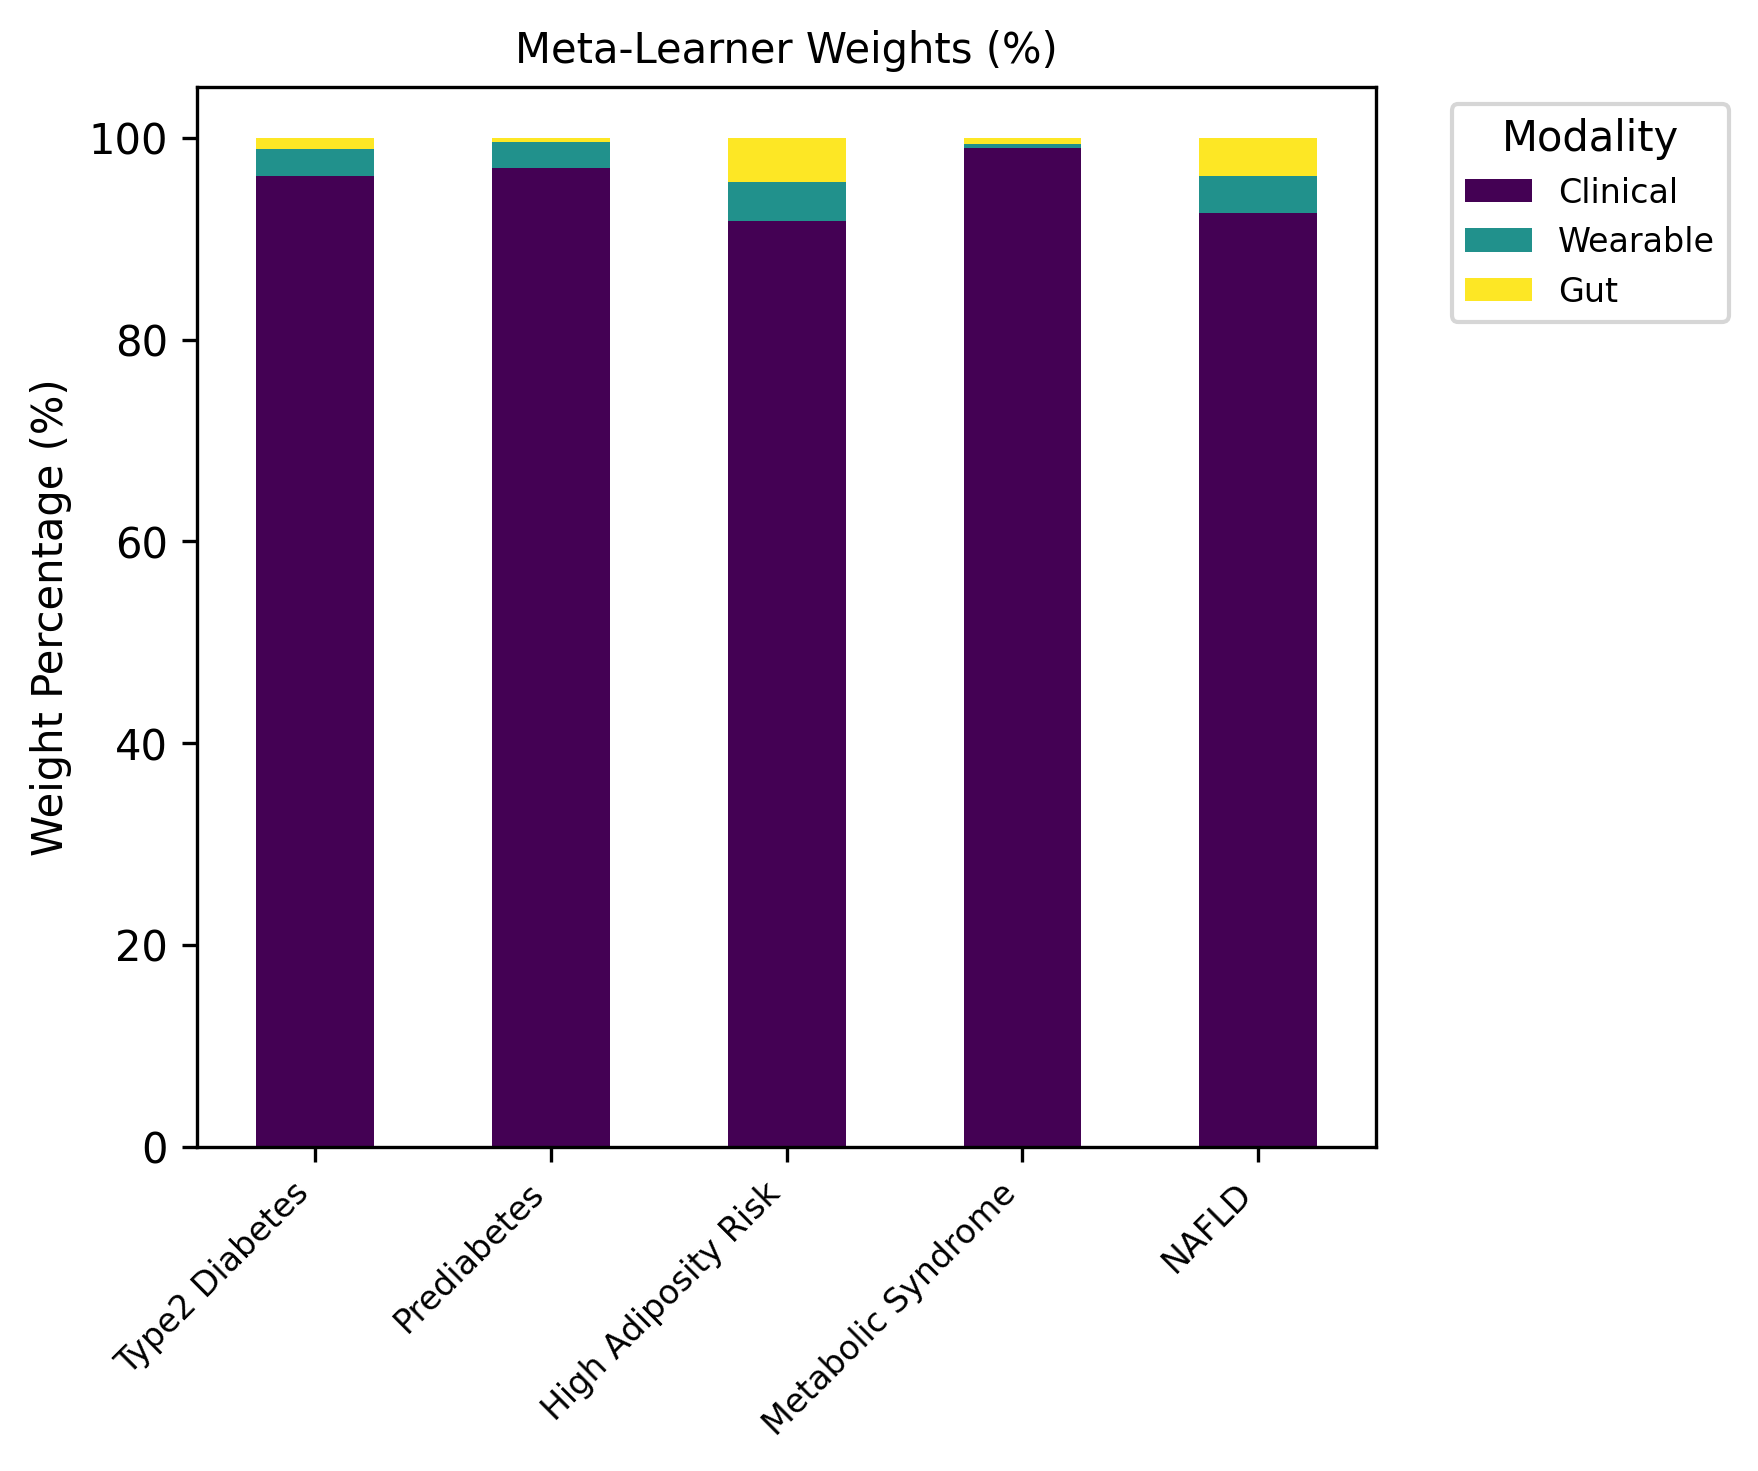
\includegraphics[width=\columnwidth]{figures/fig_meta_learner_weights.png}
\caption{Normalized Modality Attribution Weights via Meta-Learner L2 Coefficients}
\end{figure}

\section{Explainability and Medical RAG}
\subsection{TreeSHAP Methodology (RQ6)}
Unified TreeSHAP extracted localized feature attributions for all 82 variables directly from the Stage-1 expert models. Global SHAP analysis (feature importance) and local SHAP (patient-level positive/negative contributions) map how specific variables drive disease risk. However, quantitative SHAP evaluation and visual artifacts (such as global importance and patient-level waterfall plots) were not included in the current protocol.

\subsection{Medical RAG Methodology}
Using FAISS vector similarity search, patient risk factors derived from SHAP are mapped against ADA Standards of Care stored in an immutable vector database. The retrieval-grounded design is intended to reduce unsupported generation by constraining model context to retrieved evidence. RAG outputs explicitly constitute educational and lifestyle guidance. Specific implementation details (such as source document versions, chunk size, vector dimension, and top-k retrieval metrics) were not evaluated or documented in the current experimental protocol.

\section{Discussion and Limitations}
TeleMed-M3 successfully demonstrates that dynamic imputation-free routing handles arbitrary modality dropouts (RQ1) without resorting to structural numerical imputation. Ablation experiments confirm that zero-imputation routing maintains functional performance during random modality dropout significantly better than baseline median-imputation on the full multi-modal pipeline (RQ5). Performance varies heavily across modalities (RQ2), primarily because selected diagnostic-threshold relationships were intentionally encoded into the synthetic Clinical variables. Probability-level stacking with L2 regularization successfully preserves the dominant clinical signal (RQ3), and the system robustly falls back on correlational telemetry when clinical data is unavailable (RQ4). TreeSHAP and Medical RAG provide an interpretable, clinician-readable reporting structure (RQ6).

\subsection{Limitations}
The fundamental limitation of this study is the reliance on synthetically engineered data. The deterministic clinical clamping algorithms yielded artificially high baseline AUROCs that do not reflect the latent noise, measurement error, and longitudinal latency present in real-world clinical practice. Furthermore, no longitudinal or external patient validation was performed, leaving the architecture susceptible to unmeasured distribution shifts. Due to the absence of quantitative RAG evaluation, SHAP visual artifacts, and conventional numerical-imputation baselines in the current experimental protocol, no definitive claims regarding hallucination rates, clinical safety, or baseline superiority can be made. The synthetic Gut Microbiome data assumes constant-sum compositional constraints but does not substitute for true metagenomic sequencing validation. All findings remain exploratory until validated on prospective, real-world multi-omic patient cohorts.

\clearpage
\section{Conclusion}
TeleMed-M3 establishes a structurally robust imputation-free methodology for multimodal healthcare prediction. By deploying a dynamic seven-pathway router, the system leverages multi-omic physiological data when available without resorting to generative imputation when entire modalities are missing. The L2-regularized meta-learner successfully preserved the dominant Clinical signal while seamlessly incorporating correlational telemetry. Paired with Unified TreeSHAP and Medical RAG, the architecture provides a transparent, explainable foundation for Clinical Decision Support Systems. Future work will require validation of the imputation-free router on real-world longitudinal patient cohorts.

\section{Reproducibility}
All operations were locked to Seed 20260808. Models were developed using Python 3.10, scikit-learn, XGBoost, CatBoost, LightGBM, and SHAP. Models were exported as frozen \texttt{joblib} payloads (internal experiment version v4).

\bibliographystyle{IEEEtran}
\bibliography{references}

\end{document}
